%%% File encoding: UTF-8
%% äöüÄÖÜß  <-- no German Umlauts here? Use an UTF-8 compatible editor!

%%% Magic comments for setting the correct parameters in compatible IDEs
% !TeX encoding = utf8
% !TeX program = pdflatex
% !TeX spellcheck = en_US
% !BIB program = biber

\documentclass[master,english,smartquotes]{hgbthesis}
% Permissible options in [..]:
%   Type of work: diploma, master (default), bachelor, internship
%   Main language: german, english (default)
%		smartquotes: for simplified insertion of quotes (only "...")
%%%----------------------------------------------------------

\RequirePackage[utf8]{inputenc}		% Remove when using lualatex or xelatex entfernen!

\graphicspath{{img/}}    % location of images and graphics
\logofile{logo}				% logo file = images/logo.pdf (use \logofile{} for no logo)
\bibliography{references}  	% name of bibliography file (references.bib)

%%%----------------------------------------------------------
% Title page entries
%%%----------------------------------------------------------

%%% Entries for ALL types of work: --------------------------
\title{Comparing HLS with VHDL at the example of an FM Radio Receiver}
\author{Michael Wurm}

\programtype{Fachhochschul-Masterstudiengang}

\programname{Embedded Systems Design}
\placeofstudy{Hagenberg}
\dateofsubmission{2021}{07}{15}	% {YYYY}{MM}{DD}

\advisor{DI (FH) Dr. Florian Eibensteiner}	% optional

%\strictlicense		%%% restrictive license instead of Creative Commons (discouraged!)

%%%----------------------------------------------------------
\begin{document}
%%%----------------------------------------------------------

%%%----------------------------------------------------------
\frontmatter							% title part (roman page numbers)
%%%----------------------------------------------------------

\maketitle
\tableofcontents

\include{front/preface} 	% preface is optional
\chapter{Abstract}


This thesis is elaborated as the final project in the master's degree program Embedded Systems Design, at the University of Applied Sciences, Campus Hagenberg.
A comprehensive practical project is developed accompanying to the theoretical topics, which are elaborated in this thesis.\\

The main topic of this thesis is the development of a system design for an embedded system, which combines all the knowledge of different disciplines and topics, that are accumulated over the course of the entire university program.
A system-level design approach is taken to develop an FM radio receiver in multiple implementation variants, targeting a system-on-chip hardware, including an FPGA and a CPU.\\

Specifically, high-level synthesis and manual VHDL implementation is used, to develop two versions of the FPGA design.
This includes the digital signal processing chain, as well as multiple interfaces to communicate with the design.
The two variants are compared, based on specific metrics, such as implementation time, lines of code, hardware utilization, and the general usability experience during the development process.
At the end, a productive system is deployed on actual hardware, including a firmware application to provide a basic user interface.\\

The entire development process is determined by the general point of view of system design.
Therefore, a system model is developed in the first stage, by using Matlab, which allows the elaboration of algorithms for digital signal processing and the creation of a system, which can be implemented in hardware.
Furthermore, GNU Radio is used to establish a prototype, which can be deployed on actual hardware.
The entire system, with its two main implementation methods and the Matlab system model, is using a common verification environment, which guarantees a correctly functioning design.
This verification is performed in simulation and on the actual hardware, which closes the loop of the system design approach.

\chapter{Kurzfassung}

\begin{german}

Diese Masterarbeit wurde als Abschlussarbeit im Rahmen des Masterstudiengangs Embedded Systems Design an der Fachhochschule Oberösterreich, Campus Hagenberg ausgearbeitet.
Begleitend zu den theoretischen Themen dieser Arbeit wurde ein umfangreiches, praktisches Projekt entwickelt.\\

Das Hauptthema dieser Arbeit ist es, ein System-Design für ein Embedded System zu entwickeln, welches sämtliches Wissen über alle Disziplinen und Themen umfasst, die im Rahmen des Studiums behandelt wurden.
Mit einem Entwurfsansatz auf System-Ebene wird in mehreren Implementierungsvarianten ein FM Radio Empfänger entwickelt.
Zielarchitektur ist ein System-on-Chip, das aus FPGA und CPU besteht.\\

Im Speziellen werden zwei Varianten für die Implementierung eingesetzt -- High-Level Synthese und die manuelle Implementierung von VHDL Code.
Dies betrifft hauptsächlich die digitale Signalverarbeitungskette, sowie mehrere Schnittstellen, anhand welcher der Hardwareentwurf mit seiner Umgebung kommunizieren kann.
Die beiden Varianten werden anhand verschiedener Kennzahlen verglichen.
Beispielsweise werden hierfür die Zeitdauer der Implementierung, die Anzahl der Programmzeilen, die Effizienz in der Nutzung der Hardware, sowie der generelle Eindruck bezüglich der Benutzbarkeit während der Entwicklung, herangezogen.
Am Ende wird ein produktives System auf echter Hardware erstellt, inklusive einer Firmware Anwendung, um die Interaktion mit einem Benutzer zu ermöglichen.\\

Der gesamte Entwickungsprozess wird immer in dem Gesichtspunkt des Systementwurfs betrachtet.
Deshalb wird im ersten Schritt ein Systemmodell mit Matlab entwickelt.
Dieses erlaubt es, Algorithmen für die digitale Signalverarbeitung, und generell ein Gesamtsystem, zu erarbeiten, welches später in Hardware implementiert werden kann.
Weiters wird GNU Radio dazu verwendet, um einen Prototypen zu entwickeln, der bereits auf echter Hardware lauffähig ist.
Das gesamte System, inklusive der beiden Implementierungsvarianten und dem Matlab Systemmodell, verwendet eine gemeinsame Strategie und Umgebung zur Verifikation der einwandfreien Funktion des Hardwareentwurfs.
Diese Verifikation wird in Simulation, als auch direkt in der Hardware durchgeführt, wodurch sich der Kreis des Ansatzes als Systementwurf schließt.

\end{german}


%%%----------------------------------------------------------
\mainmatter          			% main part (arabic page numbers)
%%%----------------------------------------------------------

%TODO: add List of Abbreviations ??
\chapter{Introduction}
\label{cha:Introduction}

%%%%%%%%%%%%%%%%%%%%%%%
\section{Motivation}

In the master's degree program Embedded Systems Design a wide range of topics relate to digital signal processing, chip design and software development.
All of these disciplines find their application in an embedded system.
Multiple different methods of implementation are introduced for each topic and their usage is tested in practical sessions.
However, in the setting of a university course it is not always possible to look at the currently handled topic as a part of a larger, integrated system.
Instead, it is often treated as a standalone part that fulfills its own, specific functionality.

Therefore, one of the main motivation points of this thesis is to combine several disciplines and multiple implementation methods in a common context of a single project.\\

In a more general perspective, the current electronics market situation is a huge motivational factor as well.
Smart devices, smart sensors, Internet of Things (IoT) and many similar terms are well-known and are becoming more and more present in the publics' daily lives.
In some degree, all of these devices represent embedded systems, since they all consist of processing units, combined with sensors and interfaces to communicate with their outside world.
In the future, the number of devices and the range of applications in this area is going to grow from todays' point of view.
This will require a lot of engineering work to advance the state of technology we have today and explore new areas of application.\\

Since the development of an embedded system combines so many displines, it is of advantage to have knowledge of as many as possible of them.
However, not only understanding single parts, but to have an overview and understanding of the entire, integrated system and the interaction between those single parts is important in an embedded system.\\

Those major reasons lead to the choice of topic for this thesis - understanding all the single parts by themselves, while maintaining the understanding over an integrated embedded system that fulfills a task as a whole.

%%%%%%%%%%%%%%%%%%%%%%%
\section{Choice of Application}

In order to elaborate on the theoretical topics of this thesis, a comprehensive practical project is developed along with it.
The project of choice is a digital FM broadcast radio receiver.
It combines several disciplines that appear in the master's program Embedded Systems Design, such as digital signal processing (DSP), software development and system design and thus is a perfect candidate for this project.\\

FM broadcast radio is chosen as the input signal, because it is a common radio frequency signal that is available almost everywhere.
Furthermore, the demodulated signal is an audio signal, usually music or speech, that can be listened to.
This is subjectively more attractive than a generic data stream.
Additionally, it is a comparably simple signal to demodulate, but still requires several techniques of signal processing to decode it.

\section{Objective}

The main objective of this thesis is to elaborate a system design for an embedded system, that combines all the knowledge of different disciplines and topics which are accumulated over the time of the university program, in a single project.

This includes the development of a system model in a tool like Matlab, the practical usage and implementation of DSP in an FPGA, the development of a digital receiver and the deployment on actual hardware.\\

The receiver implementation on the FPGA is to be done in two variants.
The first variant is traditional, manually written hardware description language (HDL) in the programming language VHDL, as it has been done for years.
For the second variant, high-level synthesis (HLS) is employed, to generate the low-level HDL from high-level \cplusplus\ code.
These two methods are implemented and compared on the basis of usability and some metrics.

In the view of a system design approach, another focus is put on a sustainable testing and development strategy for the entire system.
Above mentioned implementation variants should optimally share as much as possible of testing and verification code, in order to save time and effort in implementation.
Also, as many tasks as possible should be automated by scripts, to save time in manual labor for the engineers working on the development.
All that enables an efficient development cycle of the product.\\

By the end of this thesis, the implementation of an FM radio receiver in multiple methods and abstraction levels should be achieved, as well as a good understanding of the overall system level design.
Knowledge of each methods' preferred field of application, efficiency and application should be gained.

%develop an FM receiver and explain it, so that it can be followed in a tutorial with an affordable budget in hardware.\\

%%%%%%%%%%%%%%%%%%%%%%%%%%%%%%%%%%%%%%%%%%%%%
% NOTES:
%%%%%%%%%%%%%%%%%%%%%%%%%%%%%%%%%%%%%%%%%%%%%
%
%Thesis Design Decisions: \\
%\\
%Main focus on system design. \\
%\\
%How to achieve the same result in 3 (4?) different levels of abstraction?
%
%\begin{enumerate}
%  \item GnuRadio (?)
%  \item Matlab/Python
%  \item HLS\\
%      Implementation targeting Xilinx' ZedBoard.\\
%      Optionally: \\
%      Intel as a comparison (synth only, no HW) - "How platform-independent is HLS?"
%  \item VHDL
%\end{enumerate}
%\vspace{.5 cm}
%
%Compare:
%- Implementation effort (difficulty)
%- Implementation time
%- Usefulness on Target Systems (uC, SoC, RasPi, etc)
%- others?

%%%%%%%%%%%%%%%%%%%%%%%%%%%%%%%%%%%%%%%%%%%%%
% FEEDBACK, Meeting 07-16-2021
%%%%%%%%%%%%%%%%%%%%%%%%%%%%%%%%%%%%%%%%%%%%%
%
%formatting:
%- absätze überall gleich (mit oder ohne leerzeile)
%references:
%- hauptsache überall gleich (Fig.2.3 oder Sec.7.1 oder Eq.3 oder Chpt.4)
%- literature refs at the beginning of a chapter/section
%  like "this chapter is based on [1][4][5]."
%  or at the end of the last sentence like "...the end of this sentence. [7]"
%
%Allgemeiner Teil / Theorie:
% zusätzliches kapitel:
%   system design ansätze
%   - from algo to VHDL (book: vom algorithmus zur hardware)
%   - matlab to VHDL
%   - systementwuf richtung test driven design
%   --> design space exploration
%
%
% ganze Arbeit aufhängen an:
%   main objective: fit all the aspects (algorithm, impl, testing) into
%                   a single project
%
%
%
%
%%%%%%%%%%%%%%%%%%%%%%%%%%%%%%%%%%%%%%%%%%%%%
% TODO General
%%%%%%%%%%%%%%%%%%%%%%%%%%%%%%%%%%%%%%%%%%%%%
%
% ## unify all graphs and diagrams
%       - all gray; use exact same gray tone; eliminate the yellow?
% ## remove old unused figures in folder img/
%

%%%%%%%%%%%%%%%%%%%%
\chapter{Signal Processing Theory}
\label{cha:TheThesis}

  \section{Modulation from Baseband to RF}
  \section{Modulation from RF to Baseband}

  \section{Frequency Modulation (FM)}
  see literature/Present\_lec6\_AM\_FM.pdf\\
  see lectures out of HSD/ESD

  Frequency modulation (FM) is a widely used standard to transmit data streams.
  The probably best known usecase therefore is commercial broadcast radio, where an audio stream is transmitted.
  Devices to receive these streams are available starting from affordable low prices to the public.


    \subsection{Mathematical description}
    \subsection{Frequency Band, Channel allocation/distribution}

  \section{Algorithms for Digital FM Demodulation}
    see literature/FmDemodulator.pdf (Sect. 3.3)
    see literature/00476180 Digital FM Demodulator for FM, TV, and Wireless.pdf (Sect. II and III)

    \subsection{Baseband Delay Demodulator}
    \subsection{Phase-Adapter Demodulator}
    \subsection{Phase-Locked Loop (PLL)}
    \subsection{Mixed Demodulator}

%%%%%%%%%%%%%%%%%%%%%%%%%%%%%%%%%%%%%%%%%%%%%%%%%%%%%%%%%%%%%%%%%%%%%%%%%%%%%%
\chapter{High-Level Synthesis}
\label{cha:HLS}

This chapter covers High-Level Synthesis in general, but also describes details that specifically apply to Xilinx.
The main sources of information for this chapter are found in \cite{VivadoUgHLSIntro}and \cite{VivadoUgHLS}.

%%%%%%%%%%%%%%%%%%%%%%%%%%%%%%%%%%%%%%%%%%%%%%%%%%%%%%%%%%%%%%%%%%%%%%%%%%%%%%
\section{Introduction}

In software development, engineers are used to writing code in a high-level language, such as C or \cplusplus.
With these languages, specific hardware details are abstracted and thus, very little knowledge of the target hardware is required.
The compiler takes over these details as it transforms the code by using the underlying, supported instruction set of the target hardware.
This has been the standard for many years by now.
In the earlier times however, it was common practise to develop programs in the low-level assembly language.
The supported instruction set of the target CPU had to be implemented directly by the software engineer.\\

A direct comparison can be drawn to FPGA design.
An FPGA engineer historically develops code in the register-transfer level (RTL), which is common practise until today.
This can be compared to developing software in the assembly language.
However, the recent development towards automation and code generation brought up High-Level Synthesis (HLS).
There, the FPGA design can be described in a high-level language, such as C or \cplusplus, which is convenient and allows to focus on the algorithm, rather than hardware details.
This high-level code is then transformed into the low-level RTL automatically, by the HLS tool.\\

The usage of HLS tries to bring software- and hardware development closer together and tries to make these two worlds more similar.
In software development, there are different compilers for multiple processor architectures, which can be used to port a program to another target hardware.
The idea of HLS is to create the same level of abstraction - write code in a high-level language, which is agnostic of its target hardware architecture.\\

A major achievement in the usage of HLS is the shorter development time.
The time that it takes to develop a first working version of the intended design can be significantly reduced, compared to the development in RTL code directly.
This is especially important when an FPGA design is combined with a software part, like in a System On Chip, since software development is comparably fast.
Fig.\ref{fig:timeline_performance_first_prototype} schematically displays the difference in development time, over performance and degree of optimization, when the same functionality of a prototype is implemented in different methods for various targets.
The compared targets are an x86 processor CPU, a digital signal processor (DSP), a graphics processing unit (GPU) and the FPGA design in RTL or HLS implementation.
It is clearly visible, that the FPGA design with the HLS design approach achieves a first working prototype much earlier than the direct RTL approach.

\includepicture [0.8] [0] {Design Time vs. Application Performance, if the same functionality is implemented in different methods for various targets \cite[Figure 1-1]{VivadoUgHLSIntro}.} {timeline_performance_first_prototype} {img/timeline_performance_first_prototype}


%%%%%%%%%%%%%%%%%%%%%%%%%%%%%%%%%%%%%%%%%%%%%%%%%%%%%%%%%%%%%%%%%%%%%%%%%%%%%%
\section{State Of The Art}

Information for this section is found in \cite{EvolutionOfHLS}, \cite{XilinxVivisHLSOpenSource} and \cite{CompareHlsVHDLArticle}.\\

HLS has been developed over 20 years ago, but has not been able to replace the manual, traditional implementation of RTL, using VHDL and Verilog, so far.
Unfortunately, no published numbers about the market share of HLS in relation to traditional implementations could be found during the research in this thesis.
However, according to the given sources it is becoming more and more popular in recent years.
This is mainly based on the fact that the HLS tools keep producing results of better quality as they are developed further.
This especially regards the efficiency of the produced RTL code, the useability of the tools, as well as the better understandable correlation between the high-level code and the generated RTL code.\\

Xilinx is the largest manufacturer of FPGAs globally and therefore its tool 'Xilinx HLS' is widely used.
Intel, the second largest FPGA manufacturer, also has its HLS tool called 'Intel oneAPI' \cite{IntelHLSOneAPI}.
Both companies are conducting serious effort to push the HLS implementation method.
Xilinx recently open-sourced the code for the front-end of their HLS compiler.
The front-end processes the HLS code, specifically \cplusplus, and creates an intermediate representation from it.
The company expects to expand the community engagement and the encouragement of innovation, driven by users, with this step.
Also Intel with its oneAPI toolkit is trying to introduce a wider usage of HLS to the community.\\

In terms of language support, several tools settle for \cplusplus.
Intel oneAPI uses library APIs and DP\cplusplus\ (Data-Parallel \cplusplus), which is an extension to the ISO \cplusplus\ standard.
Xilinx also decided in favor of the \cplusplus\ language for their tools 'Vivado HLS' and 'Vitis HLS'.
In older versions, SystemC was supported for synthesis as well, but is now deprecated in the respective latest versions \cite{VivadoHlsDeprecatesSystemC}.\\

Summing up, HLS is gaining more and more attention as it becomes more efficient.
Its usage is being promoted and pushed forward with serious effort by the major FPGA chip manufacturers and tool vendors.

%%%%%%%%%%%%%%%%%%%%%%%%%%%%%%%%%%%%%%%%%%%%%%%%%%%%%%%%%%%%%%%%%%%%%%%%%%%%%%%
%\section{Functionality}
%
%transform high-level code to HDL.\\
%-analysis\\
%-scheduling\\
%-pipelining\\
%
%- Limitations\\
%dynamic memory allocation, etc.


%%%%%%%%%%%%%%%%%%%%%%%%%%%%%%%%%%%%%%%%%%%%%%%%%%%%%%%%%%%%%%%%%%%%%%%%%%%%%%
\section{Workflow}
\label{sec:hls:workflow}

This section describes the workflow for Xilinx HLS, as it is recommended in the user guide \textit{Introduction to FPGA Design with Vivado High-Level Synthesis} \cite{VivadoUgHLSIntro}.\\

Generally, as the user guide states, the quality and the correctness of the generated output can only be as good as its input.
Consequently, it is very important to follow the design recommendations and adhere to specific rules in order to produce a high-quality input software.\\

The following list presents the main steps that are required in the implementation workflow of an HLS IP core project.\\

\begin{itemize}
  \item \textbf{Software Testbench}\\
      The developed HLS IP code needs to be verified and checked for correct functionality in a software testbench, before it gets processed to RTL code.
      This can be done by using using conventional software development tools.
      Xilinx specifically recommends dynamic code checker tools like \textit{valgrind} or \textit{Coverity}.
      They support a developer in finding memory leaks, out-of-bounds memory access, uninitialized variables and similar issues.
      Furthermore, the application of code coverage tools like \textit{gcov} is recommended as well.
      In that way, the percentage of executed code lines of testbench and HLS code can be measured, to ensure a sufficient level of testing.
      The software testbench is also called 'C Simulation'.\\

      The implementation of the HLS IP code is subject to restrictions.
      As an example, dynamic memory allocation is not supported, since the entire code must be analyzable at runtime to be processed into RTL code.
      %For further details, please read the user guides regarding Xilinx HLS.
      In contrast, the testbench code does not have any restrictions.
      Anything that is supported in C/\cplusplus\ may be used here.\\

  \item \textbf{Co-Simulation}\\
      Co-Simulation serves the purpose to verify the correct functionality of the generated RTL code.
      It is not the goal to verify the algorithm, though.
      This is already done in the previous C simulation step.
      However, the issue is that the C simulation is executed like a regular program, which means it is executed sequentially, instruction by instruction and thus parallelism cannot be represented.\\

      This is where the Co-Simulation becomes neccessary.
      The RTL code is simulated with an HDL simulator software, which can actually simulate the parallelism as it exists in the FPGA hardware.
      In that way it can be ensured, that the user did not break the functional correctness of the algorithm, by giving wrong parallelization guidance to the HLS tool.\\

      The external simulator software has to run the complex HDL simulation and return data results, which is a time consuming task.
      Therefore, the execution time of this simulation type is expected to be approximately 10.000 times slower, compared to the C simulation.\\

  \item \textbf{Integration of the generated IP}\\
      At this point, the developed HLS code is fully verified and can successfully be transformed into working RTL code.
      Xilinx HLS exports the generated RTL code in an IP structure that is supported by its IP integrator tool, that is used in Vivado or Vitis.
      Therefore, the developed IP core can be imported to the block design as another processing block, get connected with other IPs, and in that way get integrated into a larger design.\\

  \item \textbf{Synthesize FPGA bitstream}\\
      Like in any other FPGA development cycle, the created block design can now be synthesized.
      This generates a bitstream file, which can be programmed into an actual FPGA hardware.
      Depending on the architecture of the system, the developed IP may now interface with the on-chip CPU, in the example of a System-On-Chip.\\
\end{itemize}

These steps represent the standard workflow for the development of an integrated HLS IP.
A successful deployment on hardware can be achieved if they are completed accurately.
There may be more and deeper knowledge necessary, in order to use this design approach.
This thesis however focuses on system design, not on HLS specifically, and thus a comprehensive study of the referenced literature is recommended.

%%%%%%%%%%%%%%%%%%%%%%%%%%%%%%%%%%%%%%%%%%%%%%%%%%%%%%%%%%%%%%%%%%%%%%%%%%%%%%
\section{Coding}

This section gives a brief overview of some HLS-specific \cplusplus\ features that are supported with Xilinx tools.
More detailed information can be found in the respective user guide \cite{VivadoUgHLS}.

%%%%%%%%%%%%%%%%%%%%%%%%%
\subsection{Data Types}

HLS supports special data types, which are not available in standard \cplusplus.
The focus of these data types is mainly to support an optimized translation into RTL, which requires the least amount of logic cells in the FPGA.\\

Standard \cplusplus\ only supports variables in the bitwidth of byte-boundaries, so in multiples of 8 bit.
However, this may be inefficient to fit into the available FPGA target hardware.
One example therefor is the DSP48 macro that Xilinx FPGAs have built-in.
They support the multiplication of only up to 18 bit.
In an example application, the reachable number range of a variable might be limited to 17 bit for the multiplication.
However, in order to represent that, using a 32 bit data type would be necessary in standard \cplusplus.
The HLS compiler does not have this prior knowledge of the number range limit and would thus implement a 32 bit multiplication, which is a waste of resources in this case.
Because of this reason, a major feature of HLS is the possibility to define data types with arbitrary bitwidths.
In that way, the above example can be optimized to use a data type that has a bitwidth of 17 bit, which is exactly the bitwidth that is required for the application.
This results in a lower logic utilization, which in turn results in a higher maximum clock frequency that can be used.
Consequently, more functionality an be implemented in the FPGA device.
The referenced user guide shows a design example where an area reduction of 75\% is achieved by just reducing the bitwidths.\\

The argumentation is equally valid for integer data types, as well as fixed point data types.
In calculations it is often necessary to represent fractional numbers.
In standard \cplusplus, floating point data types are used therefor.
However, floating point operations require a large amount of logic to implement and thus, HLS provides fixed point data types.
These can be instantiated in arbitrary bitwidths, where integer and fractional bitwidths can be specified separately.
The fixed point format is often described in the format 'integer.fractional', like '2.14', which represents a 16 bit fixed point data type that has 2 integer bits and 14 fractional bits.\\

An example for the usage of integer and fixed point data types is given in the following code section.

\begin{CppCode}
  #include <ap_int.h>
  #include <ap_fixed.h>

  ap_int<9>   custom_integer_var1;         //  9 bit integer, signed
  ap_uint<17> custom_integer_var2;         // 17 bit integer, unsigned

  ap_fixed<16,2>  custom_fixedpoint_var1;  // 16 bit fixed point, 2.14 format, signed
  ap_ufixed<14,4> custom_fixedpoint_var2;  // 12 bit fixed point, 4.10 format, unsigned
\end{CppCode}

%%%%%%%%%%%%%%%%%%%%%%%%%
\subsection{Optimization Directives}

The HLS code can be instumented with optimization directives.
This is used to provide the HLS compiler with additional information and to instruct it on how to implement certain parts of the code in RTL.\\

Directives can be applied to interfaces, functions, loops, arrays or code regions.
They can be written in a Tcl file that is provided to the HLS project, or in the design code directly, in the form of a pre-processor pragma.
Both variants have their advantages and disadvantages.\\

Examples for such directives are optimization strategies for throughput and dataflow optimization, such as pipelining or loop unrolling.
Also the implementation of the required interface types, such as various AXI interfaces, is controlled with directives.\\

Since this topic is very comprehensive, it cannot be covered into more detail here.
For further information, refer to the user guide \cite{VivadoUgHLS}.

%%%%%%%%%%%%%%%%%%%%%%%%%
%\subsection{Optimization}
%\subsection{Functions}
%\subsection{Loops}
%\subsection{Conditional Statements}

%%%%%%%%%%%%%%%%%%%%%%%%%
\subsection{Interfaces}

Interfaces are an important asset to any IP design, since this is where they communicate with their surroundings.
This may be another IP that processes data, but may also be a CPU that reads status information or configures the IPs' settings.\\

Xilinx HLS implements two different types of interfaces: block-level, and port-level interfaces.
The block-level interface is a general interface to the IP, that can provide a handshaking functionality for when it is idle and ready to start a new operation, or when the operation is completed.
The port-level interfaces on the other hand are specific to input and output ports.
They can also provide handshaking functionality, such as data-valid indicators, acknowledge signals, or implement a FIFO for the IOs.
However, port-level interfaces can also be implemented as AXI interfaces, such as AXI4-Stream, AXI4-Lite Slave or an AXI4 Master.
This is an especially useful function, since the implementation of the actual interface logic is abstracted from the user.
Additionally, software drivers are automatically generated along with the respective interfaces, which provides a fast and simple integration into a larger system.\\

The following code example shows the specification of an AXI4-Lite memory-mapped slave interface.
The provided registers are separated into config registers and status registers.
The config is readable and writeable, while the status registers are implemented as read-only, which requires less logic in the RTL implementation.\\

\begin{program}
  \caption{Implementation of an AXI4-Lite memory-mapped slave with read-only and read-write registers.}
  \label{prog:axi4_lite}
  \begin{CppCode}
    typedef struct {
      ap_int<NUM_LEDS> led_ctrl;
      uint8_t code;
    } config_t;

    typedef struct {
      uint32_t uptime;
      uint32_t result;
    } status_t;

    void hls_ip_top_level(config_t& config,
                          status_t* status) {
        #pragma HLS INTERFACE s_axilite port = status bundle = API
        #pragma HLS INTERFACE s_axilite port = config bundle = API

        if (config.code == 0xFF) {
          status->result = 0;
          ...
        }
        ...
    }
  \end{CppCode}
\end{program}

Another code example demonstrates the equally simple definition of an AXI4-Stream interface.

\begin{CppCode}
  #include <hls_stream.h>

  void hls_ip_top_level(hls::stream<uint32_t>& sample_in,
                        hls::stream<uint32_t>& audio_out) {
      #pragma HLS INTERFACE axis port = sample_in
      #pragma HLS INTERFACE axis port = audio_out
  }
\end{CppCode}

%%%%%%%%%%%%%%%%%%%%%%%%%%%%%%%%%%%%%%%%%%%%%%%%%%%%%%%%%%%%%%%%%%%%%%%%%%%%%%
\section{Testbench}

The general significance of the simulation testbench for a HDL design is explained here, as well as the different levels of abstraction in which a HLS testbench can be executed.
These different levels of abstraction in the testbench execution are a major difference between a VHDL testbench and an HLS testbench.
The most important impact thereof is the execution speed - the time it takes to simulate a number of test cases on the DUT.\\

Section \ref{sec:hls:workflow} above already mentioned the topics of testbenches and simulation types.
The following descriptions shall be seen as a comprehensive extension around these topics.

%%%%%%%%%%%%%%%%%%%%%%%%%
\subsection{General}
\label{sub:hls:testbench:general}

In the development of software that runs on a CPU, the tool of step-by-step debugging is commonly used during the development process.
Various verification and testing libraries exist, in order to create unit tests, for example.
The advantage is, that the code that is developed there, can be compiled and run on the target CPU directly, while maintaining the direct instruction-by-instruction representation of the code.\\

However, in the development of hardware with any HDL, this is not possible.
HDL languages provide a syntax and semantic representation that allow to create parallel structures and a dependency on timing, such as a system clock.
The design is based on signals that perform logic operations and transfer values into registers.
Thus, HDL code is often called register-transfer level, or short, RTL code.
Before this code can be run on the target hardware, i.e. an FPGA, it needs to run through a process called synthesis.
In synthesis, the HDL code is translated into a netlist and is consequently mapped into hardware logic cells that are available in the target device.
Various optimizations are done during this process, so that the direct connection to the code representation is lost.
Additionally, it is impossible to access every single signal within the design during debugging on the hardware, which is probably also one of the main issues.
Synthesis tools like Xilinx Vivado provide support to make debugging possible in hardware, but require a large effort to implement them, especially in terms of synthesis time.
Another big factor that speaks against debugging in hardware generally, is that the process of synthesis takes a comparably large amount of time to transform code into the target technology.
Each time the code is adapted, the entire synthesis process needs to be started over again.
Because of all of these reasons, debugging HDL code step-by-step as in software is not possible.\\

Thus, in order to allow debugging and verification of HDL code, the technology of simulation was invented.
Here, the HDL is also translated into a netlist that represents all the parallel processes just like in hardware, but the subsequent step of synthesis is not taken.
Therefore, simulation comes to a result much faster.
Since HDL designs actually only consist of electrical wires and some basic block primitives, like flipflops or lookup tables, it is difficult to verify correct values.
They would need to be compared in their binary bit-pattern format, at the correct point in time.
Of course the HDL language provides support with different datatypes, that abstract the binary number representation and make the numbers human-readable.
However, it remains an enormous effort to manually write testing code to verify a bus interface, for example.
In order to simplify such complex operations, various testbench frameworks and libraries are available to developers.

%%%%%%%%%%%%%%%%%%%%%%%%%
\subsection{C Simulation}

In C Simulation, the HLS compiler is used to create an executable binary that includes the testbench code, as well as the IP design of the DUT.
This binary can be run just like any other program.
The most important note here is, that the HLS code is \textit{not} transformed into RTL at this point.
Instead, the HLS code is treated as a regular \cplusplus\ code, that uses some libraries, like the fixed-point library.
This means, that the HLS IP cores' top-level function is used as a regular function call in the testbench.\\

The main advantage of this type of simulation is the major increase of execution speed.
The reason for this speed-up is the abstraction of timing, such as clock cycles or similar constraints.
In fact, there is absolutely no timing information that needs to be taken into account in this simulation.

%%%%%%%%%%%%%%%%%%%%%%%%%
\subsection{C/RTL Co-Simulation}

This type of simulation actually transforms the HLS IP code into RTL code, such as Verilog or VHDL, for the testbench.
This is done in three steps.\\

\begin{itemize}
  \item \textbf{Create input vectors}\\
  In this first step, the above explained, regular C simulation is executed.
  Hereby, the inputs that are sent to the DUT are stored as 'input vectors'.

  \item \textbf{Perform RTL simulation}\\
  Next, the previously generated input vectors are applied to the DUT.
  At this point, the DUT is already translated into RTL code, so the code that is used here is either VHDL or Verilog code.
  The default simulator is the Vivado Simulator (XSim).
  However, various other simulators like ModelSim are supported.
  The generated outputs of this step are stored as 'output vectors'.
  \item \textbf{Verify the results}\\
  The final verification step sources the output vectors back to the C testbench, which compares the outputs with the expected results.\\
\end{itemize}

\noindent
This type of simulation takes a significantly longer time to execute, because timing information now actually needs to be considered for the RTL code.

%%%%%%%%%%%%%%%%%%%%
\chapter{System Architecture and Concept}
\label{cha:SystemArchitectureAndConcept}

This chapter introduces the FM radio receiver project that is implemented as a major part of this thesis.
It specifically talks about the system level approach that is taken in the implementation of the project.
The main concept, as well as the architecture are explained.

%%%%%%%%%%%%%%%%%%%%
\section{Overview}

In the development of a project that includes multiple functional parts, it is always of advantage to start with a system level overview.
Major decisions can be made at this stage, before any implementation has begun.
This can have a direct impact on the efficiency of the entire development, which concequently has an impact on the final quality of the product.
A thorough system level design can also prevent from issues that would otherwise arise while the development is already ongoing.
As an example it could turn out that one of the functional parts is not able to fit into the integrated system, in the way it is implemented.
This leads to the necessity to re-engineer this entire functional block.
As a result, it takes more effort to implement the functionality, which directly correlates with the development cost and the time-to-market, in order to deliver the final product.
Summing up, a comprehensive system level architecture and concept can pave the way for a successful implementation of a project from start to finish.\\

In order to create a system level design, considerations around the high-level, final goal of the product are a good starting point.
This includes the definition of its functional range.
Once this is done, the target system or target hardware should be considered, because there are various ways to implement a certain functionality.
All of these variants will eventually result in the same output, but will, however, heavily differ in their implementation effort, efficiency, or their applicability for the products' aim in general.
Thus, things like the available hardware platform, implementation time, degree of optimization, output quality, and similar things are important factors at this stage.
Of course, there are many more factors to consider when a product is to be developed.
However, only a subset of these is covered here, since this chapter is focused on how this thesis' accompanying project was developed and is thus written in that context.\\

%%%%%%%%%%%%%%%%%%%%
\section{The project}

The aim of this thesis is develop a system architecture and concept, that allows the implementation of an FM radio receiver in multiple different ways, while providing an elegant way to compare the different solutions.
The final goal thereby is always be the same, that is: Listen to the music of a radio station that is transmitted over FM broadcast radio.

In the context of a system level design approach, several steps are necessary to find a solution that is ready to be implemented.
As a very first step, the inner workings of an FM receiver need to be understood.
This mainly regards the signal processing theory, to be able to decode the signal that is received by the antenna.
Chapter \ref{cha:SignalProcessingTheory} describes this part into detail.

As already mentioned above, multiple ways of technology and implementation can lead to a similar result.
Thus, the next step is to define a set of possible ways, which will actually be implemented.
For this thesis, the decision was made to implement the FM radio receiver, using the following methods.

\begin{itemize}
  \item \textbf{GNU Radio}\\
      GNU Radio is a free and open-source software development toolkit to implement a software-defined radio.
      The implementation is done by connecting functional blocks in a block design.
      This abstracts the inner workings of each functional block and thus provides an implementation approach on a very high level of abstraction.
      GNU Radio supports interfaces to external RF hardware \cite{SoftwareGnuRadio}.
  \item \textbf{Matlab}\\
      Matlab is a software platform that can work with matrices and compute numerical solutions.
      Matlab also includes various toolboxes, that support developers with complex calculations and tasks on datasets.
      This includes a range of toolboxes for signal processing, such as filter designers or FFT functions, as well as convenient ways to visualize data \cite{SoftwareMatlab}.
  \item \textbf{FPGA: \cplusplus High-Level Synthesis}\\
      In order to use an FPGA, a hardware design needs to be developed for it.
      This can be done using high-level synthesis.
      High-level synthesis (HLS) is explained in detail in Chapter \ref{cha:HLS}.
  \item \textbf{FPGA: VHDL}\\
      Similar to the HLS approach, this is a variant to write a hardware design for an FPGA.
      The language VHDL is used in this approach.
\end{itemize}

In order to implement an FM radio receiver, all of the listed methods require deep knowledge about the neccessary details of signal processing.
However, the implementation of the various different methods require more or less knowledge and effort on the exact underlying implementation of each signal processing part.
This depends on their level of abstraction.

%-  implementation of a model and DSP concept in Matlab \\
%-  implementation in VHDL and HLS \\
%-  both use the same testbench source \\
%-  both are integrated into FPGA
%-  the FPGA output is read back into the firmware, for analysis \\

%%%%%%%%%%%%%%%%%%%%
\section{Block Diagram}



%%%%%%%%%%%%%%%%%%%%
\subsection{describe blocks}

%%%%%%%%%%%%%%%%%%%%
\section{Test Environment}

%%%%%%%%%%%%%%%%%%%%
\chapter{Implementation}
\label{cha:Implementation}

This chapter describes the most important details of each implementation variant.

\section{Digital Signal Processing Chain}

\includepicture [1.0] {Detailed block diagram of the digital signal processing chain.} {bd_dsp_detailed} {img/bd_detailed_dsp}

\section{Matlab Model}

in fixed point, close to hardware level algorithm

\subsection{Transmitter block diagram}

\section{GNU Radio}
  \subsection{Introduction}
  \subsection{Transmitter}
  \subsection{Receiver}

\section{VHDL (no shortcut)}
  \subsection{Testbench}
  \subsection{Channel Selection (IF to Channel-BB)}
  \subsection{Phase Detector}
  \subsection{other Elements}

  \section{High-Level Synthesis}
  \subsection{Testbench}
  \subsection{Channel Selection (IF to Channel-BB)}
  \subsection{Phase Detector}
  \subsection{other Elements}

\section{Common Testbench}
  \subsection{Architecture (same tb for VHDL and HLS-generated HDL)}
  \subsection{Framework cocotb, with ghdl compiler}
  Instantiate both HDL models in the testbench.\\
  Display a direct comparison of outputs in graphs. This is practical, since the cocotb framework runs in python and graphs can be generated using Python's matplotlib.


%%%%%%%%%%%%%%%%%%%%
\chapter{Deployment on Hardware}
\label{cha:DeploymentOnHardware}

This chapter describes the additional parts of implementation that are necessary in order to run the implemented FM radio on actual hardware.
The hardware that is used is introduced as well.

%%%%%%%%%%%%%%%%%%%%
\section{GNU Radio}

The GNU Radio implementations, both receiver and transmitter, are used in combination with external hardware.
The specific hardware that is used is briefly described here.\\

In order to interface with the real world, two different hardware devices are used.
Both devices are supported by GNU Radio and are briefly described here.

%%%%%%%%%%%%%%%%%%%%
\subsection{Ettus Research USRP b200mini}

The USRP b200mini is a device that can be used to create a software-defined radio.
It resembles the size of a business card and is developed by Ettus Research.
A signal range from 70 MHz to 6 GHz can be covered by the front end.
The board further features a Xilinx Spartan-6 FPGA that is user-programmable, which makes the device very flexible for various applications with the received signal \cite{USRPb200Mini}.\\

GNU Radio supports this device with the blocks \textit{UHD: USRP Sink} and \textit{UHD: USRP Source}.
Therefore, it can be used as both a receiver and a transmitter.

%%%%%%%%%%%%%%%%%%%%
\subsection{RTL-SDR}

The RTL-SDR is a cheap USB dongle, that was originally developed as a DVB-T TV tuner.
It is based on the RTL2832U chipset, which includes an 8-bit ADC and a digital signal processor.
The device delivers IQ data via the USB interface \cite{RTLSDR}.\\

\noindent
Based on its hardware, the RTL-SDR can only be used as a receiver.


%%%%%%%%%%%%%%%%%%%%
\section{FPGA Hardware Platform}

The ZedBoard is a development board that is developed by Xilinx.
It is specifically designed around the Xilinx Zynq-7000 SoC, which contains a dual-core ARM Cortex A9 processor core and a programmable logic, the FPGA.
The board further offers a range of features from external DDR3 memory, over various connectors, such as RJ45 Ethernet, USB, 3.5 mm audio, HDMI, Pmod, buttons to LEDs and a display.\\

The most important features for this project are the audio line-out connector and the SD card port.
Additionally, the LEDs are used to display various status information during runtime of the FM receiver.

\includepicture [0.75] [0] [H] {The ZedBoard PCB \cite{ZedBoard}.} {zedboard_photo} {img/zedboard_photo}

%%%%%%%%%%%%%%%%%%%%
\section{System-On-Chip Design}

Chapter \ref{cha:Implementation} already described the development of the main IP core, which is the FM radio receiver in the VHDL and HLS variants.
In order to embed this IP on actual FPGA, or rather SoC hardware, a significant additional amount of implementation is neccessary.
In this section, these additional parts of the implementation, which specifically enable and support the deployment on hardware, are described.

%%%%%%%%%%%%%%%%%%%%
\subsection{Architecture}

The block diagram in Fig.\ref{fig:bd_impl_vivado} shows the implemented architecture that is used in the SoC.
The various design domains in and around the SoC are depicted in different visual representations.
The FPGA domain blocks are highlighted in gray.
The processor system domain is shown as white blocks.
Blocks that are external to the SoC are drawn with dashed lines.

\includepicture [1.0] {Block diagram of the Vivado implementation.} {bd_impl_vivado} {img/draw.io/bd_impl_vivado}

%%%%%%%%%%%%%%%%%%%%
\subsection{Functionality}
%TODO: re-work this section for better wording
%TODO: refer to above theory chapters, with verification and HIL, etc..
The FM receiver IP is the main functionality of the design.
However, the design around it needs to function properly in order for the IP to work correctly, which is explained in the following passage.\\

The CPU is the main actor that determines any actions on the system.
It reads a file from the external SD card and stores this data in a dedicated memory area.
Next, the DMA is configured and a continuous transfer mode is initiated, so that the data in the mentioned memory area is transferred into the FPGA in a loop.
Any data connection in the following IP block chain is implemented as an AXI stream bus.
The first block after the DMA is an AXI Stream Switch.
It can switch its single input to be forwarded to either of the outputs.
The switch is configured by the CPU, to enable one output at a time.
Consequently, one of the FM radio receiver IPs is provided with data, which is processed to produce an audio output.
This audio output data is delivered to another AXI Stream Switch, that fulfills the function to either select the output of above or below IP, in coordination with the first switch, obviously.
The next block is an AXI Stream Broadcaster, which takes a single stream input and simply duplicates it at its output, so that the outputs are an exact copy of the input.
One of these duplicates is sourced to an AXI-Stream-To-I2S converter, which generates the I2S signals for the external audio codec chip.
The second duplicate is connected to a FIFO, which simply stores the generated output data.
The FIFO asserts an interrupt to the CPU, on which it reads out the entire FIFO buffer.
The CPU then stores this data on the external SD card again.
In that way, the loop of data is closed, which enables the verification of the respective IPs correct functionality.
Therefore, this system design can be described as a hardware-in-the-loop system, in the point of view of the FPGA IPs.\\

It is to note, that Xilinx provides all the AXI infrastructure IPs, and thus the only self-implemented IPs are the FM radio receivers, as well as the I2S interface.
Nevertheless, the correct design and implementation of the architecture still needs to be formulated by the user.

%%%%%%%%%%%%%%%%%%%%
\subsection{Software}

drivers for IPs, libraries to interface with e.g. SD card, etc\\
--> look at software which parts may be interesting to highlight

%%%%%%%%%%%%%%%%%%%%
\chapter{Comparison and Results}
\label{cha:ComparisonAndResults}

This chapter presents the results that are achieved in the development of the FM Radio Receiver project, with the chosen different methods.
However, the main focus is to compare the results that are achieved with HLS and VHDL, since these are the major implementation variants of the project.

%%%%%%%%%%%%%%%%%%%%%%%%%%%%%%%%%%%%%%%%%%%%%%%%%%%%%%%%%%%%%%%%%%%%%%%%%%%%%%
\section{General}

A main objective of this thesis is to implement an FM radio receiver in multiple different methods.
This includes GNU Radio, Matlab, VHDL and HLS, which all have their advantages and disadvantages and surface different challenges to the developer.
The target functionality is to listen to the audio broadcast signal of an FM radio station.\\

All of the listed methods are implemented and the target functionality is achieved with all of them.
However, the level of detail that is required in the implementation, and the resulting effort and time it takes to implement the respective variant, differs by a large factor.
This is mainly due to the different levels of abstraction, so that the low-level algorithms do not need to be known.\\

In the following sections, especially the HLS and VHDL implementations are compared on the basis of metrics, but also based on the experience during development.


%%%%%%%%%%%%%%%%%%%%%%%%%%%%%%%%%%%%%%%%%%%%%%%%%%%%%%%%%%%%%%%%%%%%%%%%%%%%%%
\section{Functionality}

Generally, both tools -- HLS and VHDL -- provide the capabilities to implement any functionality in one or the other method.
However, the implementation is done in a different level.
VHDL uses an approach that is very close to the hardware, such as clock cycles and flipflops, while HLS describes the logic on an algorithmic level.\\

The implementation is split into two main parts, the communication interfaces and the DSP.
The results are presented in the following sections.

% Functionality same?
% DSP yes, AXI no (FSM of axi-stream)
% unit tests

%%%%%%%%%%%%%%%%%%%%
\subsection{Interfaces}

The AXI4-Lite memory-mapped bus is implemented to have an exactly equal behaviour in both variants.
There are read-only and read-writeable registers, which are all mapped onto a single base address.\\

The AXI stream interface however does not show the exact same behaviour.
Here, the HLS variant is using the AXI stream according to its protocol, while the VHDL variant is implemented differently.
It uses a simplified logic for the ready-flag, which reduces the effort in implementation.
However, from the perspective of the communicating blocks, the interface is usable like a regular AXI stream.
The implementation details are explained in Section \ref{sec:impl:vhdl:interfaces}.\\

In the final, integrated system on the SoC hardware, the CPU is able to communicate with both IPs via their interfaces successfully.
Status and configuration data can be read and written through the AXI4-Lite interface, and the streaming data for the DSP chain is successfully sent through the AXI streams as well.

%%%%%%%%%%%%%%%%%%%%
\subsection{Audio Output}

The audio output of the HLS and VHDL variants is compared with the Matlab model, which serves as the reference.
Additionally, the results of the testbench are compared with their respective result in the actual hardware.
In summary, it can be stated that the DSP chain produces a very similar audio output in all the compared data sets.
However, differences remain, which are presented in the following paragraphs and diagrams.

\includepicture [1.0] [0] {Comparison of the IP audio output signals, in simulation and hardware, against the Matlab model. The HLS variant matches the model, while the VHDL output diverts by a certain amount. Also, VHDL differs between simulation- and hardware results.} {audio_output_compare_tb_vs_hw} {img/matlab/audio_output_compare_tb_vs_hw}

%%%%%
\subsubsection{Comparing against the Matlab reference}

In the comparison against the Matlab model, the HLS variant achieves a very exact match of the output signal.
However, the VHDL implementation differs by a certain amount.
There seems to be an issue in the signal separation between the left and right audio channels.
This is visible in the analysis of the audio signal, as shown is Figure \ref{fig:audio_output_compare_tb_vs_hw}.
The signal strength of the left channel in the upper diagram is weaker than expected, while the right channel in the lower diagram is stronger.
This imbalance can also be observed by listening to the audio output via speakers.\\

The cause for this issue may be located in several components in the design.
This includes the FM demodulator, the carrier recovery, i.e. the 38~kHz carrier, as well as a sample timing shift in the final summation and substraction to recover the left and right channels.
The FIR filter has a successfully passing unit test and is thus assumed to be correct.
Also the fixed-point data type with its overflow- and rounding behaviour is suspected to be a potential issue.
Due to the time limitation in the elaboration of this thesis, this issue can not be traced down to the root cause and thus still persists in the current implementation.
However, from the system-level point of view of this thesis, the IP works and can be integrated into the final system.

%\includepicture [1.0] [0] {Comparison of the IP audio output signals against the Matlab model. The HLS variant matches the model, while the VHDL output diverts by a certain amount.} {audio_output_compare_ips_vs_matlab} {img/matlab/audio_output_compare_ips_vs_matlab}

%%%%%
\subsubsection{Comparing simulation- against hardware results}

Here, the results of the simulation testbenches are compared against the values that are read from the FPGA directly.
Ideally, the values should be exactly the same.
However, Figure \ref{fig:audio_output_compare_tb_vs_hw} shows that this is not always the case.
Again, the HLS implementation does have a matching result, whereas the VHDL variant has deviating values.
The explanation here may be linked with above suspicions, but may also be linked to the initial reset values that exist in the hardware.
In the HLS implementation, the reset logic of several registers is implemented automatically, whereas in VHDL these conditions need to be implemented manually.
Therefore, the IPs internal state, i.e. the register values, may be different at the beginning, which leads to an error propagation throughout the design.
The entire DSP chain is built like a pipeline and therefor it takes a number of samples to process, before the 'wrong' intermediate values are flushed out.
All that may be the cause for the deviating values in the VHDL design.\\

Again, the time limitation in the elaboration of this thesis does not allow a deeper analysis and investigation of this issue.
However, the end-to-end system design enables the developer to analyze an issue like this in a convenient way, in quick iterations.
Any adaptions in the VHDL design can be simulated and integrated into the FPGA with automated scripts.
Both results can then be analyzed and compared, which may lead to further adaptions.\\


%%%%%%%%%%%%%%%%%%%%%%%%%%%%%%%%%%%%%%%%%%%%%%%%%%%%%%%%%%%%%%%%%%%%%%%%%%%%%%
\section{Code Development}

In the development of a software project, the metric for the lines of code is sometimes used to give an idea of the complexity of the project.
The time it takes to implement a certain set of features can also give such an insight, even though it is a subjective metric, since it is influenced by the respective delopers experience.
However, both metrics are applied to the FM Radio Receiver project.

%%%%%%%%%%%%%%%%%%%%
\subsection{Lines of Code}

Several parts of the system design are taken into account to analyze the lines of code, to give an impression over the largest code parts in the project.

\includepicture [0.9] [0] {Lines of code of the respective system design parts, presented in a pie chart.} {lines_of_code_pie_chart} {img/matlab/lines_of_code_pie_chart_py}

\begin{figure}%
  \centering
  \subfloat[\centering label 1]{{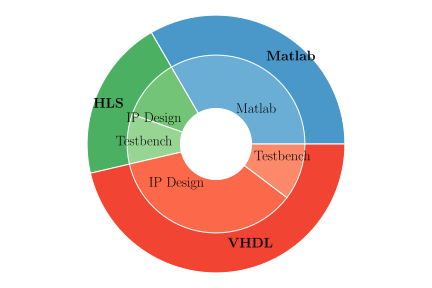
\includegraphics[trim=10 10 10 10,clip, width=0.45\textwidth]{img/matlab/lines_of_code_pie_chart_py} }}%
  \\
  %\hspace{\fill}
  \subfloat[\centering label 2]{{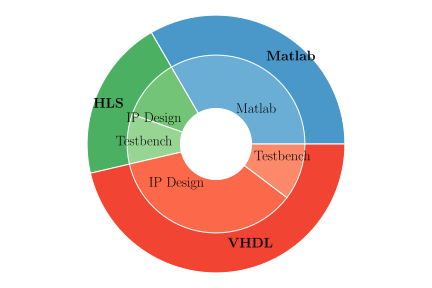
\includegraphics[trim=10 10 10 10,clip, width=0.45\textwidth]{img/matlab/lines_of_code_pie_chart_py} }}%
  %\hspace{\fill}
  %\vspace{3cm}
  \subfloat[\centering label 3]{{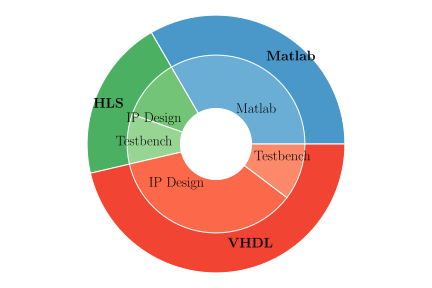
\includegraphics[trim=10 10 10 10,clip, width=0.45\textwidth]{img/matlab/lines_of_code_pie_chart_py} }}%

  \caption{Multiple Figures side by side}%
  \label{fig:example}%
\end{figure}


%\begin{GenericCode}
%Matlab:
%  Language     files blank comment code TotalWithoutBlank Total
%  ____________ _____ _____ _______ ____ _________________ _____
%  MATLAB          34   551     728 1451              2179  2730
%
%VHDL IP Design:
%  Language     files blank comment code TotalWithoutBlank Total
%  ____________ _____ _____ _______ ____ _________________ _____
%  VHDL            20   525     787 1431              2218  2743
%  Python           1    45      22  141               163   208
%
%VHDL Testbench:
%  Language     files blank comment code TotalWithoutBlank Total
%  ____________ _____ _____ _______ ____ _________________ _____
%  Python           5   141     141  426               567   708
%  make             2    19      18   70                88   107
%  Bourne Shell     1     5       6   16                22    27
%
%HLS IP Design:
%  Language     files blank comment code TotalWithoutBlank Total
%  ____________ _____ _____ _______ ____ _________________ _____
%  C/C++ Header    14    90     119  221               340   430
%  C++              9    97     197  195               392   489
%
%HLS Testbench:
%  Language     files blank comment code TotalWithoutBlank Total
%  ____________ _____ _____ _______ ____ _________________ _____
%  C++              1    39      44  141               185   224
%  Tcl/Tk           5    33      37  112               149   182
%  C/C++ Header     2    24      18   87               105   129
%  make             1    24      26   69                95   119
%  Python           1    19      21   45                66    85
%\end{GenericCode}


%%%%%%%%%%%%%%%%%%%%
\subsection{Implementation Time}

% Implementation effort/time
%    -- see logged times; is subjective; had no previous knowledge
%    -- AXI interfaces --> huge effort in VHDL...
%        (mention Johannes Walter for generously providing/allowing the Register Engine script, adapted for this thesis)
%    -- drivers are auto-generated with HLS! huge time-saving..
%       (maybe show the code of AXI4-Lite interface and its generated driver
%        --> difference between R/W and RO!;
%        and show screenshots of the IP in the block design)

%%%%%%%%%%%%%%%%%%%%%%%%%%%%%%%%%%%%%%%%%%%%%%%%%%%%%%%%%%%%%%%%%%%%%%%%%%%%%%
\section{Simulation}
% Sim speed of x min of recorded FM signal
%
% VHDL:
%          time                samples
%   audio         sim        in      out
%  0.1000 s    73:44 min  (96000 -> 4000)
%  0.0100 s    09:37 min  ( 9600 ->  400)
%  0.0025 s    02:36 min  ( 2400 ->  100)
%
% HLS:



%%%%%%%%%%%%%%%%%%%%%%%%%%%%%%%%%%%%%%%%%%%%%%%%%%%%%%%%%%%%%%%%%%%%%%%%%%%%%%
\section{System Design}

The system design architecture that is chosen in this project covers several parts of the system.
This includes a reference model, the development of the IP itself, including the simulation testbench, as well as the final integration into the productive system.
Because of this structured approach, that is given by this system design, it can be applied to almost any DSP project.
The main processing IP can simply be replaced with another implementation, while the environment does not need to be modified.
The reason therefor is, that DSP projects almost always use streaming interfaces for their inputs and outputs.
Also a configuration interface is commonly used, to adapt certain parameters of the IP during runtime.


%%%%%%%%%%%%%%%%%%%%%%%%%%%%%%%%%%%%%%%%%%%%%%%%%%%%%%%%%%%%%%%%%%%%%%%%%%%%%%
\section{Deployment on Hardware}

%%%%%%%%%%%%%%%%%%%%
\subsection{Integration}
% IP generation and integration into Vivado

%%%%%%%%%%%%%%%%%%%%
\subsection{Hardware Utilization}
% --> utilization reports

%%%%%%%%%%%%%%%%%%%%
\subsection{Latency}
% --> utilization reports

%%%%%%%%%%%%%%%%%%%%%%%%%%%%%%%%%%%%%%%%%%%%%%%%%%%%%%%%%%%%%%%%%%%%%%%%%%%%%%
\section{Applicability}
% of all implementation variants
%   GNU Radio for fast prototyping,
%   Matlab for research
%   HLS/VHDL for deployment on HW, product development




%%%----------------------------------------------------------
\appendix                                         % appendix
%%%----------------------------------------------------------

\include{back/appendix_a}	% technical supplements
\include{back/appendix_b}	% contents of the CD-ROM/DVD

\backmatter
\chapter{List of Abbreviations}
\label{cha:listabbrev}

\begin{tabbing}
\hspace{25 mm}\=\kill

\textbf{ADC}       \> Analog Digital Converter\\
\textbf{AM}        \> Amplitude Modulation\\
\textbf{AXI}       \> Advanced Extensible Interface\\
\textbf{BP}        \> Bandpass (Filter)\\
\textbf{CI}        \> Continuous Integration\\
\textbf{CPU}       \> Central Processing Unit\\
\textbf{DC}        \> Direct Current\\
\textbf{DSB-SC}    \> Dual-Sideband Suppressed-Carrier\\
\textbf{DUT}       \> Device Under Test\\
\textbf{ERP}       \> Effective Radiated Power\\
\textbf{FM}        \> Frequency Modulation\\
\textbf{FPGA}      \> Field-programmable Gate Array\\
\textbf{HDL}       \> Hardware Description Language\\
\textbf{HLS}       \> High-Level Synthesis\\
\textbf{IF}        \> Intermediate Frequency\\
\textbf{IoT}       \> Internet of Things\\
\textbf{IP}        \> Intellectual Property\\
\textbf{IQ, I/Q}   \> Inphase and Quadrature components\\
\textbf{LED}       \> Light Emitting Diode\\
\textbf{LP}        \> Lowpass (Filter)\\
\textbf{LSB}       \> Least Significant Bit\\
\textbf{LNA}       \> Low Noise Amplifier\\
\textbf{LO}        \> Local Oscillator\\
\textbf{PM}        \> Phase Modulation\\
\textbf{RTL}       \> Register Transfer Level\\
\textbf{RDS}       \> Radio Data System\\
\textbf{SDR}       \> Software Defined Radio\\
\textbf{SoC}       \> System On Chip\\
\textbf{USB}       \> Universal Serial Bus\\
\textbf{VHDL}      \> Very High Speed Integrated Circuit Hardware Description Language\\
\textbf{VHF}       \> Very High Frequency\\

\end{tabbing}


%\addcontentsline{toc}{chapter}{\listfigurename}
%\listoffigures

%%%----------------------------------------------------------
\MakeBibliography                        				% references
%%%----------------------------------------------------------

%%% special page for checking print size --------------------
\include{back/printbox}

%%%----------------------------------------------------------
\end{document}
%%%----------------------------------------------------------
